\section{层流非定常流动算例}\label{sec:appendix-d-2}

\begin{example}[单位正方形上给定解、齐次 Dirichlet 边界条件的非定常算例]\label{ex:appendix-d-7}
考虑 $\Omega=(0,1)^2$,取以下给定解:
\begin{equation}\label{eq:appendix-d-24}
\begin{aligned}
\bm u&=2\pi\sin(t)
\begin{pmatrix}
\sin^2(\pi x)\sin(\pi y)\cos(\pi y)\\
-\sin(\pi x)\cos(\pi x)\sin^2(\pi y)
\end{pmatrix},\\
p&=20\sin(t)\left(x^2y-\frac16\right).
\end{aligned}
\end{equation}
时刻 $t=1.7$ 的解见图\hyperref[fig:appendix-d-7]{D.7}.按定义,$\bm u|_{\partial\Omega}=0$.给定黏度后,选取右端项 $\bm f$,使式\hyperref[eq:appendix-d-24]{(D.24)}满足 Navier--Stokes 方程\hyperref[eq:dimensionless-ns-standard]{(2.25)}.
\begin{elegantfigure}[0.88\linewidth]
 \includegraphics[page=766,pagebox=cropbox,trim=52.50bp 464.90bp 52.36bp 60.25bp,clip,width=\linewidth]{../input/source/Finite Element Methods for Incompressible Flow Problems.pdf}
 \captionof{figure}{例题 D.7:$t=1.7$ 时计算得到的解.}\label{fig:appendix-d-7}
\end{elegantfigure}
该测试问题可用于支持误差估计.为了覆盖式\hyperref[eq:appendix-d-24]{(D.24)}中的时间增长和衰减阶段,终止时间应足够长,例如\textcite{deFrutos2016c} 所取的 $T=5$.
\end{example}

\begin{example}[定常入口下 $\mathrm{Re}=100$ 的非定常圆柱绕流]\label{ex:appendix-d-8}
该算例描述层流 Kármán 涡街.其设置与例题\hyperref[ex:appendix-d-5]{D.5} 非常相似:计算区域、黏度、圆柱及通道上下壁面的边界条件、出口的 do-nothing 条件\hyperref[eq:appendix-d-13]{(D.13)}以及体力 $\bm f=0$ 均相同.唯一变化是入口速度增至式\hyperref[eq:appendix-d-12]{(D.12)}的五倍:
\begin{equation}\label{eq:appendix-d-25}
\bm v(0\,\mathrm m,y)
=\frac{1}{0.41^2}
\begin{pmatrix}6y(0.41-y)\\0\end{pmatrix}
\frac{\mathrm m}{\mathrm s},
\qquad 0\,\mathrm m\le y\le0.41\,\mathrm m.
\end{equation}
因此,与例题\hyperref[ex:appendix-d-5]{D.5}相比,特征速度尺度和 Reynolds 数也增大五倍,分别为 $U_{\mathrm{mean}}=1\,\mathrm{m/s}$ 和 $\mathrm{Re}=100$.此时问题不存在稳定稳态解,故应以非定常不可压缩 Navier--Stokes 方程\hyperref[eq:time-dependent-ns-strong]{(7.1)}为模型.采用与例题\hyperref[ex:appendix-d-5]{D.5}相同的特征尺度,无量纲黏度为 $\nu=10^{-3}$.

此问题需要初始条件,但不存在解析形式的初始解.可先用任意初始条件启动模拟,继续计算直至 Kármán 涡街形成并趋于周期状态.达到这一状态后,保存某一离散时刻的数值解,并将其作为后续模拟的初始条件.

与例题\hyperref[ex:appendix-d-5]{D.5}类似,感兴趣的量是圆柱所受阻力系数、升力系数,以及圆柱前后压力差.与稳态问题不同,动量方程还含速度的时间导数.由式\hyperref[eq:appendix-d-5]{(D.5)}和\hyperref[eq:appendix-d-8]{(D.8)}可得
\begin{equation}\label{eq:appendix-d-26}
\begin{aligned}
c_{\mathrm{drag}}=-20\Bigl[&(\partial_t\bm u,\bm w_{\mathrm{drag}})
+(\nu\nabla\bm u,\nabla\bm w_{\mathrm{drag}})\\
&+n(\bm u,\bm u,\bm w_{\mathrm{drag}})
-(\nabla\cdot\bm w_{\mathrm{drag}},p)\Bigr].
\end{aligned}
\end{equation}
\begin{equation}\label{eq:appendix-d-27}
\begin{aligned}
c_{\mathrm{lift}}=-20\Bigl[&(\partial_t\bm u,\bm w_{\mathrm{lift}})
+(\nu\nabla\bm u,\nabla\bm w_{\mathrm{lift}})\\
&+n(\bm u,\bm u,\bm w_{\mathrm{lift}})
-(\nabla\cdot\bm w_{\mathrm{lift}},p)\Bigr].
\end{aligned}
\end{equation}
其中 $\bm w_{\mathrm{drag}}$ 和 $\bm w_{\mathrm{lift}}$ 的定义见例题\hyperref[ex:appendix-d-5]{D.5}.时间导数项可用后向差分近似,例如
\[
(\partial_t\bm u,\bm w_{\mathrm{drag}})
\approx \frac{1}{\Delta t_{n+1}}
(\bm u^{n+1}-\bm u^n,\bm w_{\mathrm{drag}}).
\]
压力降按式\hyperref[eq:appendix-d-18]{(D.18)}计算.图\hyperref[fig:appendix-d-8]{D.8}给出了阻力系数、升力系数和压力降的典型变化.
\begin{elegantfigure}[0.92\linewidth]
 \includegraphics[page=767,pagebox=cropbox,trim=53.00bp 86.40bp 53.11bp 308.75bp,clip,width=\linewidth]{../input/source/Finite Element Methods for Incompressible Flow Problems.pdf}
 \captionof{figure}{例题 D.8:感兴趣的量随时间的变化.}\label{fig:appendix-d-8}
\end{elegantfigure}

另一个感兴趣的泛函是 Strouhal 数\hyperref[eq:dimensionless-parameters]{(2.23)},它与周期长度密切相关(式\hyperref[eq:dimensionless-parameters]{(2.23)}中的 $T^*$ 表示周期长度).实际中,可以由阻力系数或升力系数的极值位置,或由升力系数的零点,估计周期长度.模拟一段时间后,对连续若干周期的长度取平均.
表\hyperref[tab:appendix-d-2]{D.2}列出\textcite{SchaeferTurek1996} 给出的感兴趣量参考区间.这里 $t_{0,\mathrm{per}}$ 是某一周期的起始时刻(升力系数达到极大值时),$T_{\mathrm{per}}$ 为周期长度.
\begin{eleganttable}
\captionof{table}{例题 D.8 的参考区间.}\label{tab:appendix-d-2}
\begin{tabular}{lc}
\toprule
量 & 参考区间\\
\midrule
$c_{\mathrm{drag,max}}$ & $[3.22,3.24]$\\
$c_{\mathrm{lift,max}}$ & $[0.98,1.02]$\\
$\Delta p(t_{0,\mathrm{per}}+T_{\mathrm{per}}/2)$ & $[2.46,2.50]$\\
Strouhal 数 & $[0.295,0.305]$\\
\bottomrule
\end{tabular}
\par\smallskip
\parbox{0.9\linewidth}{\centering 参考区间据\textcite{SchaeferTurek1996}.}
\end{eleganttable}
\end{example}

\begin{example}[时变入口下 Reynolds 数介于 $0$ 与 $100$ 的非定常圆柱绕流]\label{ex:appendix-d-9}
该算例描述涡脱落的产生和衰减,其设置与例题\hyperref[ex:appendix-d-5]{D.5}几乎相同,只有入口边界条件不同:
\begin{equation}\label{eq:appendix-d-28}
\begin{aligned}
\bm v(t',0,y)
&=\sin\left(\frac{\pi t'}{8\,\mathrm s}\right)
\frac{1}{0.41^2}
\begin{pmatrix}6y(0.41-y)\\0\end{pmatrix}
\frac{\mathrm m}{\mathrm s},\\
&\qquad y\in[0,0.41]\,\mathrm m,\quad t'\in[0,8]\,\mathrm s.
\end{aligned}
\end{equation}
其频率为 $\Omega=\pi\,\mathrm{s}^{-1}$.该算例的入口平均速度为
\[
U_{\mathrm{mean}}(t')
=\sin\left(\frac{\pi t'}{8\,\mathrm s}\right)
\frac{\int_0^{0.41}6y(0.41-y)\,\mathrm dy}
     {0.41^2\int_0^{0.41}\mathrm dy}
\frac{\mathrm m}{\mathrm s}
=\sin\left(\frac{\pi t'}{8\,\mathrm s}\right)\frac{\mathrm m}{\mathrm s}.
\]
以圆柱直径 $d=0.1\,\mathrm m$、入口平均速度及运动黏度 $\mu/\rho$ 为尺度,该流动的 Reynolds 数满足 $0\le\mathrm{Re}(t')\le100$.出口可采用与式\hyperref[eq:appendix-d-28]{(D.28)}相应的 Dirichlet 条件
\begin{equation}\label{eq:appendix-d-29}
\begin{aligned}
\bm v(t',2.2\,\mathrm m,y)
&=\sin\left(\frac{\pi t'}{8\,\mathrm s}\right)
\frac{1}{0.41^2}
\begin{pmatrix}6y(0.41-y)\\0\end{pmatrix}
\frac{\mathrm m}{\mathrm s},\\
&\qquad y\in[0,0.41]\,\mathrm m,\quad t'\in[0,8]\,\mathrm s.
\end{aligned}
\end{equation}
也可采用 do-nothing 条件
\begin{equation}\label{eq:appendix-d-30}
\bm S(t')\bm n
=\bigl(2\mu D(\bm v)(t')-P(t')I\bigr)\bm n
=\bm0\,\mathrm{N/m^2}
\quad\text{于 }\Gamma_{\mathrm{out}},\quad t'\in[0,8]\,\mathrm s.
\end{equation}
初始条件取 $\bm v_0=0\,\mathrm{m/s}$.图\hyperref[fig:appendix-d-9]{D.9}展示了不同时刻的流场.
\begin{elegantfigure}[0.92\linewidth]
 \includegraphics[page=769,pagebox=cropbox,trim=52.50bp 236.90bp 52.36bp 60.25bp,clip,width=\linewidth]{../input/source/Finite Element Methods for Incompressible Flow Problems.pdf}
 \captionof{figure}{例题 D.9:速度场的时间演化,分别显示 $2$、$4$、$5$、$6$、$7$ 和 $8$ 秒时的结果.}\label{fig:appendix-d-9}
\end{elegantfigure}

无量纲入口条件为
\[
\begin{aligned}
\bm u(0,y)
&=\sin\left(\frac{\pi t}{8}\right)
\frac{1}{0.41^2}
\begin{pmatrix}6y(0.41-y)\\0\end{pmatrix},\\
&\qquad 0\le y\le0.41,\quad t\in[0,8].
\end{aligned}
\]
与例题\hyperref[ex:appendix-d-5]{D.5}一样,感兴趣的量为阻力系数\hyperref[eq:appendix-d-3]{(D.3)}、升力系数\hyperref[eq:appendix-d-6]{(D.6)}及圆柱前后压力差
\[
\Delta P(t)=P(t,0.15,0.2)-P(t,0.25,0.2).
\]
由于有限元三角剖分无法精确表示圆周边界,阻力和升力应采用面积积分公式\hyperref[eq:appendix-d-5]{(D.5)}和\hyperref[eq:appendix-d-8]{(D.8)},而不是边界积分公式\hyperref[eq:appendix-d-4]{(D.4)}和\hyperref[eq:appendix-d-7]{(D.7)}.这些公式中取 $U=1\,\mathrm{m/s}$、$L=1\,\mathrm m$、$A=0.1\,\mathrm m$、$V=U_{\mathrm{mean}}(4\,\mathrm s)=1\,\mathrm{m/s}$,便得到式\hyperref[eq:appendix-d-26]{(D.26)}和\hyperref[eq:appendix-d-27]{(D.27)}.

\textcite{JohnRang2010} 对感兴趣的量计算了精确度较高的参考曲线,见图\hyperref[fig:appendix-d-10]{D.10}.这些曲线对应出口采用 Dirichlet 条件\hyperref[eq:appendix-d-29]{(D.29)}的情形.表\hyperref[tab:appendix-d-3]{D.3}列出参考值.
\begin{elegantfigure}[0.92\linewidth]
 \includegraphics[page=770,pagebox=cropbox,trim=52.50bp 168.90bp 53.61bp 225.50bp,clip,width=\linewidth]{../input/source/Finite Element Methods for Incompressible Flow Problems.pdf}
 \captionof{figure}{例题 D.9:据\textcite{JohnRang2010}给出的感兴趣量参考曲线.}\label{fig:appendix-d-10}
\end{elegantfigure}
\begin{eleganttable}
\captionof{table}{例题 D.9 的参考值.}\label{tab:appendix-d-3}
\begin{tabular}{lcc}
\toprule
量 & 数值 & 时刻\\
\midrule
$c_{\mathrm{drag,max}}^{\mathrm{ref}}$ & $2.950918381$ & $3.93625$\\
$c_{\mathrm{lift,max}}^{\mathrm{ref}}$ & $0.47787543$ & $5.69250$\\
$\Delta p(8\,\mathrm s)^{\mathrm{ref}}$ & $-0.11161567$ & \\
\bottomrule
\end{tabular}
\par\smallskip
\parbox{0.9\linewidth}{\centering 参考值据\textcite{JohnRang2010}.}
\end{eleganttable}
\end{example}

\begin{example}[二维和三维指数衰减流动:Beltrami 流]\label{ex:appendix-d-10}
设 $\Omega\subset\mathbb R^3$,考虑以下速度场和压力场族:
\begin{equation}\label{eq:appendix-d-31}
\bm u=-\alpha e^{-\nu\gamma^2t}
\begin{pmatrix}
e^{\alpha x}\sin(\alpha y+\gamma z)+e^{\alpha z}\cos(\alpha x+\gamma y)\\
e^{\alpha y}\sin(\alpha z+\gamma x)+e^{\alpha x}\cos(\alpha y+\gamma z)\\
e^{\alpha z}\sin(\alpha x+\gamma y)+e^{\alpha y}\cos(\alpha z+\gamma x)
\end{pmatrix},
\end{equation}
\[
\begin{aligned}
p=-\frac{\alpha^2}{2}e^{-2\nu\gamma^2t}\bigl[&
e^{2\alpha x}+e^{2\alpha y}+e^{2\alpha z}\\
&+2\sin(\alpha x+\gamma y)\cos(\alpha z+\gamma x)e^{\alpha(y+z)}\\
&+2\sin(\alpha y+\gamma z)\cos(\alpha x+\gamma y)e^{\alpha(z+x)}\\
&+2\sin(\alpha z+\gamma x)\cos(\alpha y+\gamma z)e^{\alpha(x+y)}
\bigr]+C.
\end{aligned}
\]
这里 $\alpha,\gamma\in\mathbb R$ 是用户选取的参数,见图\hyperref[fig:appendix-d-11]{D.11}.若在 $\partial\Omega$ 上施加 Dirichlet 边界条件,则常数 $C$ 应选得使 $p$ 的积分平均值为零.将式\hyperref[eq:appendix-d-31]{(D.31)}代入 Navier--Stokes 方程\hyperref[eq:time-dependent-ns-strong]{(7.1)},直接计算可得 $\bm f=0$.这族解由\textcite{EthierSteinman1994} 推导,其构造依据以下原则:
\begin{itemize}
  \item 速度场应无散;
  \item 时间导数应与黏性项平衡,即 $\partial_t\bm u-\nu\Delta\bm u=0$;
  \item 对流项应能表示为某个标量函数的梯度,且该梯度与压力梯度互相抵消,即 $(\bm u\cdot\nabla)\bm u+\nabla p=0$.
\end{itemize}
直接计算可得
\begin{equation}\label{eq:appendix-d-32}
\nabla\times(\nabla\times\bm u)=0.
\end{equation}
满足性质\hyperref[eq:appendix-d-32]{(D.32)}的流称为 Beltrami 流.图\hyperref[fig:appendix-d-11]{D.11}展示了 $t=0$ 时 $\alpha=\pi/4$、$\gamma=\pi/2$ 的速度和压力.
\begin{elegantfigure}[0.92\linewidth]
 \includegraphics[page=771,pagebox=cropbox,trim=52.50bp 116.40bp 52.36bp 411.50bp,clip,width=\linewidth]{../input/source/Finite Element Methods for Incompressible Flow Problems.pdf}
 \captionof{figure}{例题 D.10:区域 $\Omega=(-1,1)\times(-1,1)\times(0,2)$ 上 $t=0$ 时的速度和压力,参数取 $\alpha=\pi/4$、$\gamma=\pi/2$.}\label{fig:appendix-d-11}
\end{elegantfigure}

\textcite{Taylor1923} 早已提出二维区域 $\Omega=(0,\pi)^2$ 上的指数衰减流动问题:
\[
\bm u=e^{-2\nu t}
\begin{pmatrix}
-\cos x\sin y\\
\sin x\cos y
\end{pmatrix},
\qquad
p=-\frac14e^{-4\nu t}\bigl(\cos(2x)+\cos(2y)\bigr).
\]
例如,\textcite{Chorin1968} 对这类解进行了数值研究.
\end{example}

\begin{note}[时变入口下三维 $\mathrm{Re}\in[0,100]$ 圆柱绕流]\label{note:appendix-d-11}
\textcite{SchaeferTurek1996} 还定义了例题\hyperref[ex:appendix-d-9]{D.9} 的三维扩展,其设置与例题\hyperref[ex:appendix-d-6]{D.6} 相似.与后者相比,该问题的入口速度随时间变化,且在大部分时间区间内更强.然而,\textcite{John2006} 发现该算例不会发生涡脱落.由于缺少这一流动特征,采用此算例的意义有限.
\end{note}
